\chapter{Priority Queues}

\tikzset{
  hn/.style={circle,draw,minimum size=6.5mm,inner sep=0pt,font=\small},
  ac/.style={draw,minimum width=8mm,minimum height=7mm}
}

\section{Abstract Data Types}

\begin{definition}
An \emph{abstract data type} (ADT) describes a collection of data and the
operations on it, without saying how it is stored. A \emph{data structure} is a
concrete implementation of an ADT.
\end{definition}

Familiar examples: a \emph{stack} (LIFO; \code{push}, \code{pop}) and a
\emph{queue} (FIFO; \code{enqueue}, \code{dequeue}), both implementable with
arrays or linked lists so that every operation is $\Theta(1)$ (amortized for a
dynamic array).

\section{The Priority Queue ADT}

\begin{definition}
A \emph{priority queue} stores items, each with a \emph{priority} (key), and
supports
\begin{itemize}
  \item \code{insert(x)}: add item $x$ with its priority;
  \item \code{deleteMax()}: remove and return an item of highest priority.
\end{itemize}
(A min-oriented priority queue uses \code{deleteMin} instead.) Optional extras:
\code{size}, \code{isEmpty}, \code{getMax}.
\end{definition}

Stacks and queues are special cases (priority = insertion time, or its negative).

\subsection{PQ-Sort}

Any priority queue gives a sorting algorithm:
\begin{lstlisting}
PQ-Sort(A[0..n-1]):
  PQ <- empty priority queue
  for k <- 0 to n-1 do PQ.insert(A[k])
  for k <- n-1 down to 0 do A[k] <- PQ.deleteMax()
\end{lstlisting}
The running time is $\bigO(n \cdot \text{insert} + n \cdot \text{deleteMax})$.

\subsection{Simple Implementations}

\begin{center}
\begin{tabular}{llll}
\toprule
Implementation & \code{insert} & \code{deleteMax} & PQ-Sort is\ldots\\
\midrule
Unsorted array/list & $\Theta(1)$ & $\Theta(n)$ & selection sort, $\Theta(n^2)$\\
Sorted array/list & $\Theta(n)$ & $\Theta(1)$ & insertion sort, $\Theta(n^2)$\\
Binary heap & $\Theta(\log n)$ & $\Theta(\log n)$ & heapsort, $\Theta(n\log n)$\\
\bottomrule
\end{tabular}
\end{center}

\section{Binary Heaps}

\begin{definition}
A (max-)\emph{heap} is a binary tree satisfying
\begin{enumerate}
  \item \textbf{Structural property:} every level is full except possibly the
        last, which is filled from the left.
  \item \textbf{Heap-order property:} for every node $v$ other than the root,
        $\text{key}(\text{parent}(v)) \ge \text{key}(v)$.
\end{enumerate}
\end{definition}

Consequently the maximum is at the root. The heap is \emph{not} sorted: siblings
are in no particular order.

\begin{lemma}
A heap with $n$ nodes has height $\Theta(\log n)$.
\end{lemma}
\begin{proof}
If the height is $h$, levels $0, \ldots, h-1$ are full, so
$n \ge 2^h$; and the tree has at most $2^{h+1} - 1$ nodes. Thus
$2^h \le n \le 2^{h+1} - 1$, so $h = \floor{\log_2 n}$.
\end{proof}

\subsection{Array Storage}

Because of the structural property, store the nodes level by level, left to
right, in an array $A[0..n-1]$. No pointers are needed:
\begin{itemize}
  \item root at $A[0]$;
  \item children of $A[i]$ at $A[2i+1]$ and $A[2i+2]$;
  \item parent of $A[i]$ ($i > 0$) at $A[\floor{(i-1)/2}]$;
  \item the last node is $A[n-1]$.
\end{itemize}

\begin{example}
The array $[50, 29, 34, 27, 15, 8, 10, 23, 26]$ is a heap: e.g.\ $A[1] = 29$ has
children $A[3]=27$ and $A[4]=15$; $A[3]=27$ has children $23$ and $26$.

\begin{center}
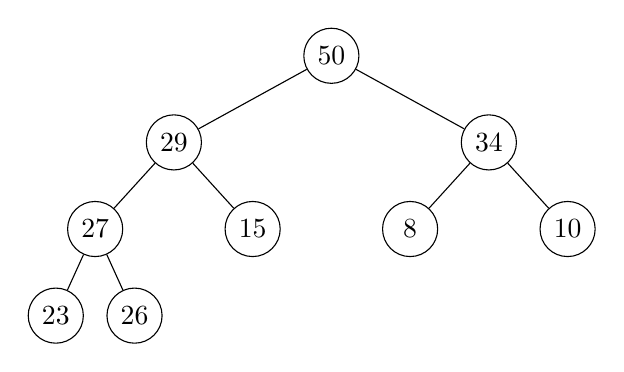
\begin{tikzpicture}[level distance=1.1cm,
  level 1/.style={sibling distance=4cm},
  level 2/.style={sibling distance=2cm},
  level 3/.style={sibling distance=1cm},
  every node/.style={circle,draw,minimum size=7mm,inner sep=1pt}]
\node {50}
  child {node {29}
    child {node {27} child {node {23}} child {node {26}}}
    child {node {15}}}
  child {node {34}
    child {node {8}}
    child {node {10}}};
\end{tikzpicture}
\end{center}
In the array, each node's arrows go to its children at indices $2i+1$ (blue) and
$2i+2$ (orange):
\begin{center}
\begin{tikzpicture}
  \node[ac] (a0) at (0.0,0) {50};
  \node[font=\scriptsize,gray] at (0.0,-0.6) {0};
  \node[ac] (a1) at (0.8,0) {29};
  \node[font=\scriptsize,gray] at (0.8,-0.6) {1};
  \node[ac] (a2) at (1.6,0) {34};
  \node[font=\scriptsize,gray] at (1.6,-0.6) {2};
  \node[ac] (a3) at (2.4,0) {27};
  \node[font=\scriptsize,gray] at (2.4,-0.6) {3};
  \node[ac] (a4) at (3.2,0) {15};
  \node[font=\scriptsize,gray] at (3.2,-0.6) {4};
  \node[ac] (a5) at (4.0,0) {8};
  \node[font=\scriptsize,gray] at (4.0,-0.6) {5};
  \node[ac] (a6) at (4.8,0) {10};
  \node[font=\scriptsize,gray] at (4.8,-0.6) {6};
  \node[ac] (a7) at (5.6,0) {23};
  \node[font=\scriptsize,gray] at (5.6,-0.6) {7};
  \node[ac] (a8) at (6.4,0) {26};
  \node[font=\scriptsize,gray] at (6.4,-0.6) {8};
  \draw[-{Stealth},blue!60!black] (a0.north) to[out=60,in=120] (a1.north);
  \draw[-{Stealth},orange!80!black] (a0.north) to[out=60,in=120] (a2.north);
  \draw[-{Stealth},blue!60!black] (a1.north) to[out=60,in=120] (a3.north);
  \draw[-{Stealth},orange!80!black] (a1.north) to[out=60,in=120] (a4.north);
  \draw[-{Stealth},blue!60!black] (a2.north) to[out=60,in=120] (a5.north);
  \draw[-{Stealth},orange!80!black] (a2.north) to[out=60,in=120] (a6.north);
  \draw[-{Stealth},blue!60!black] (a3.north) to[out=60,in=120] (a7.north);
  \draw[-{Stealth},orange!80!black] (a3.north) to[out=60,in=120] (a8.north);
\end{tikzpicture}
\end{center}
\end{example}

\subsection{Insertion: fix-up (bubble-up)}

Place the new item in the next free spot (preserving structure), then swap it
upward while it is larger than its parent.
\begin{lstlisting}
insert(x):
  A[n] <- x; n <- n + 1
  fix-up(A, n-1)

fix-up(A, k):
  while k > 0 and A[parent(k)] < A[k] do
    swap A[k] and A[parent(k)]
    k <- parent(k)
\end{lstlisting}
Each swap moves up a level, so the time is $\bigO(\text{height}) = \bigO(\log n)$.

\begin{center}
\begin{tikzpicture}
  \begin{scope}[level distance=0.95cm,level 1/.style={sibling distance=3.0cm},level 2/.style={sibling distance=1.5cm},level 3/.style={sibling distance=0.75cm}]
  \node[hn] (b0) {50} child {node[hn,fill=yellow!25] (b1) {29} child {node[hn] (b3) {27} child {node[hn] (b7) {23}} child {node[hn] (b8) {26}}} child {node[hn,fill=yellow!25] (b4) {15} child {node[hn,fill=orange!30] (b9) {45}} child[missing]}} child {node[hn] (b2) {34} child {node[hn] (b5) {8}} child {node[hn] (b6) {10}}};
  \end{scope}
  \draw[-{Stealth},thick,red!70!black] (b9) to[bend right=40] (b4);
  \draw[-{Stealth},thick,red!70!black] (b4) to[bend right=30] (b1);
  \node[font=\scriptsize] at (0,0.7) {insert 45 at $A[9]$, then fix-up};
  \draw[-{Stealth},thick] (3.4,-1.5) -- (4.4,-1.5);
  \begin{scope}[xshift=7.8cm,level distance=0.95cm,level 1/.style={sibling distance=3.0cm},level 2/.style={sibling distance=1.5cm},level 3/.style={sibling distance=0.75cm}]
  \node[hn] (c0) {50} child {node[hn,fill=orange!30] (c1) {45} child {node[hn] (c3) {27} child {node[hn] (c7) {23}} child {node[hn] (c8) {26}}} child {node[hn] (c4) {29} child {node[hn] (c9) {15}} child[missing]}} child {node[hn] (c2) {34} child {node[hn] (c5) {8}} child {node[hn] (c6) {10}}};
  \end{scope}
  \node[font=\scriptsize] at (7.8,0.7) {after two swaps ($45 < 50$: stop)};
\end{tikzpicture}
\end{center}

\subsection{deleteMax: fix-down (bubble-down)}

Remove the root, move the last item to the root, then swap it down with its
\emph{larger} child while it is smaller than that child.
\begin{lstlisting}
deleteMax():
  max <- A[0]
  swap A[0] and A[n-1]; n <- n - 1
  fix-down(A, n, 0)
  return max

fix-down(A, n, k):
  while k is not a leaf do       // 2k+1 < n
    j <- 2k+1                    // left child
    if j+1 < n and A[j+1] > A[j] then j <- j+1
    if A[k] >= A[j] then break
    swap A[k] and A[j]
    k <- j
\end{lstlisting}
Again $\bigO(\log n)$.

\begin{important}[Pitfall]
In fix-down you must swap with the \emph{larger} child; swapping with the smaller
one breaks heap order between the two children.
\end{important}

\begin{example}
\code{deleteMax} on the heap above: return 50, move 26 to the root, giving
\[[26, 29, 34, 27, 15, 8, 10, 23].\]
The larger child of 26 is 34: swap, giving
\[[34, 29, 26, 27, 15, 8, 10, 23].\]
Now 26 at index 2 has children 8, 10: stop.
\begin{center}
\begin{tikzpicture}
  \begin{scope}[level distance=0.95cm,level 1/.style={sibling distance=3.0cm},level 2/.style={sibling distance=1.5cm},level 3/.style={sibling distance=0.75cm}]
  \node[hn,fill=orange!30] (d0) {26} child {node[hn] (d1) {29} child {node[hn] (d3) {27} child {node[hn] (d7) {23}} child[missing]} child {node[hn] (d4) {15}}} child {node[hn,fill=yellow!25] (d2) {34} child {node[hn] (d5) {8}} child {node[hn] (d6) {10}}};
  \end{scope}
  \draw[{Stealth}-{Stealth},thick,red!70!black] (d0) to[bend left=30] (d2);
  \node[font=\scriptsize] at (0,0.7) {26 moved to the root};
  \draw[-{Stealth},thick] (3.4,-1.5) -- (4.4,-1.5);
  \begin{scope}[xshift=7.8cm,level distance=0.95cm,level 1/.style={sibling distance=3.0cm},level 2/.style={sibling distance=1.5cm},level 3/.style={sibling distance=0.75cm}]
  \node[hn] (e0) {34} child {node[hn] (e1) {29} child {node[hn] (e3) {27} child {node[hn] (e7) {23}} child[missing]} child {node[hn] (e4) {15}}} child {node[hn,fill=orange!30] (e2) {26} child {node[hn] (e5) {8}} child {node[hn] (e6) {10}}};
  \end{scope}
  \node[font=\scriptsize] at (7.8,0.7) {swapped with the larger child 34};
\end{tikzpicture}
\end{center}
\end{example}

\section{Building a Heap: Heapify}

Given $n$ items in an array, we want to make it a heap.

\paragraph{Option 1 (top-down):} insert items one at a time with fix-up. Worst
case $\Theta(n \log n)$ (e.g.\ sorted increasing input: every item bubbles to
the root).

\paragraph{Option 2 (bottom-up, Floyd):} treat the array as a tree and call
fix-down on each internal node, from the last internal node back to the root.
\begin{lstlisting}
heapify(A, n):
  for i <- parent(n-1) down to 0 do
    fix-down(A, n, i)
\end{lstlisting}
When we fix-down at node $i$, both subtrees of $i$ are already heaps, so
afterward the subtree at $i$ is a heap (by induction).

\begin{theorem}
Bottom-up heapify runs in $\Theta(n)$ time.
\end{theorem}
\begin{proof}[Proof sketch]
Let $h = \floor{\log n}$. A node at height $j$ (distance $j$ from the bottom)
costs $\bigO(j)$ in fix-down, and there are at most $\ceil{n/2^{j+1}}$ nodes at
height $j$. So the total is
\[
\sum_{j=0}^{h} \frac{n}{2^{j+1}} \cdot \bigO(j)
= \bigO\!\left(n \sum_{j \ge 0} \frac{j}{2^{j}}\right) = \bigO(2n) = \bigO(n).
\]
Clearly $\Omega(n)$ since every item is touched.
\end{proof}

Intuition: most nodes are near the bottom, and those nodes only travel a short
distance. In top-down insertion most nodes are near the bottom and travel a
\emph{long} distance.

\begin{example}
Heapify $[3, 1, 6, 5, 2, 4]$. Internal nodes are indices $2, 1, 0$.
\begin{itemize}
  \item $i = 2$ (6): child 4; $6 \ge 4$, no change.
  \item $i = 1$ (1): children 5, 2; swap with 5: $[3,5,6,1,2,4]$.
  \item $i = 0$ (3): children 5, 6; swap with 6: $[6,5,3,1,2,4]$; then 3 at index
        2 has child 4; swap: $[6,5,4,1,2,3]$.
\end{itemize}
\end{example}

\section{HeapSort}

\begin{lstlisting}
HeapSort(A, n):
  heapify(A, n)                 // Theta(n)
  while n > 1 do
    swap A[0] and A[n-1]        // move max to its final position
    n <- n - 1
    fix-down(A, n, 0)
\end{lstlisting}
\begin{itemize}
  \item Time: $\Theta(n) + n \cdot \bigO(\log n) = \bigO(n \log n)$, and it is
        $\Theta(n \log n)$ in the worst case.
  \item Space: \emph{in place}, $\Theta(1)$ auxiliary space (the heap shrinks as
        the sorted suffix grows).
  \item Not stable.
\end{itemize}

\section{Other Heap Uses}

\paragraph{Finding the $k$-th largest.} Heapify then $k$ deleteMax calls:
$\bigO(n + k \log n)$. Alternatively keep a min-heap of size $k$ while scanning:
$\bigO(n \log k)$. (Chapter 3 does this in $\Theta(n)$ expected time.)

\paragraph{Merging $k$ sorted lists.} Keep the heads of the lists in a min-heap
of size $k$; total $\bigO(n \log k)$.

\begin{aside}
Other PQ realisations exist (meldable heaps, binomial heaps) that also support
efficient \code{merge}; a randomized meldable heap merges two heaps in expected
$\bigO(\log n)$ by recursively merging into a randomly chosen subtree. Some terms
covered these briefly as enrichment.
\end{aside}

\section{Summary}
\begin{itemize}
  \item Priority queue ADT: \code{insert}, \code{deleteMax}. Any PQ gives a sort.
  \item A binary heap is a nearly complete binary tree with heap order, stored
        in an array with index arithmetic.
  \item \code{insert} (fix-up) and \code{deleteMax} (fix-down) take $\bigO(\log n)$.
  \item Bottom-up heapify is $\Theta(n)$ because $\sum j/2^j$ converges.
  \item HeapSort: $\Theta(n \log n)$ worst case, in place, not stable.
\end{itemize}
